\section{Resultados}

\begin{frame}
\frametitle{Resultados}

\begin{itemize}
  \item \textbf{Taxa de Acertos:}  a raz�o entre a quantidade de caracter�sticas
  corretamente localizadas e o n�mero de caracter�sticas na imagem inicial
  \item \textbf{An�lise de Tempo:} os usu�rios n�o toleram aplica��es com
menos do que 5fps
\end{itemize}

\end{frame}



\newcommand{\gtype}{pres}


\newcommand{\minscale}{0.2}
\newcommand{\maxscale}{1.2}
\newcommand{\minangle}{0}
\newcommand{\maxangle}{30}
\newcommand{\minblur}{0}
\newcommand{\maxblur}{4}
\newcommand{\minbright}{-50}
\newcommand{\maxbright}{50}
\newcommand{\correctmatches}{0.6}
\newcommand{\cadencia}{200}
\newcommand{\maxtime}{10000}


\newcommand{\miny}{-10}
\newcommand{\maxy}{3}
\newcommand{\minx}{-150}
\newcommand{\maxx}{400}
\newcommand{\ylimit}{0.6}
\newcommand{\ylabel}{Percent of correct matches}
\newcommand{\graphwidth}{0.7}



\subsection{Taxa de Acertos}


\begin{frame}
\begin{figure}[H]
\centering

%scale 
\begin{tikzpicture}
	\pgfplotsset{small}
\begin{axis}
	[
	   width=\graphwidth\textwidth,
    ylabel=$\ylabel$, % Set the labels
    xlabel=$Scale Factor$,
	legend entries={$BRISK$,$FAST$,$FREAK$,$GFTT$,$MSER$,$ORB$,$STAR$,$SURF$,$SIFT$},
	legend pos=outer north east,
	title= Robustness to scaling
    ]
	\addplot table [x=Argument, y=BRISK    , col sep=comma]	{graphs/scale-all-\gtype.csv}; 
	\addplot table [x=Argument, y=FAST     , col sep=comma]	{graphs/scale-all-\gtype.csv}; 
	\addplot table [x=Argument, y=FREAK    , col sep=comma]	{graphs/scale-all-\gtype.csv}; 
	\addplot table [x=Argument, y=GFTT     , col sep=comma]	{graphs/scale-all-\gtype.csv};
	 \addplot table [x=Argument, y=MSER     , col	sep=comma]	{graphs/scale-all-\gtype.csv};
	  \addplot table [x=Argument, y=ORB      , col sep=comma]	{graphs/scale-all-\gtype.csv}; 
	\addplot table [x=Argument, y=STAR     , col sep=comma]	{graphs/scale-all-\gtype.csv}; 
	\addplot table [x=Argument, y=SURF     , col sep=comma]	{graphs/scale-all-\gtype.csv}; 
	\addplot table [x=Argument, y=SIFT     , col sep=comma]	{graphs/scale-all-\gtype.csv}; 
	
	
	%eixo horizontal
	\addplot[red,sharp plot,update limits=false] coordinates{(\minx,\ylimit)(\maxx,\ylimit)};
	 \fill [opacity=0.4,red!25] (axis	cs:\minx,\miny)	rectangle (axis	
	 cs:\maxx,\ylimit);
	
	
	%eixo vertical
	\addplot[blue,sharp plot,update limits=false] coordinates {(\minscale,\miny)(\minscale,\maxy)} ;
		\fill [opacity=0.4,blue!25] (axis cs:0,-1) rectangle (axis	cs:\minscale,\maxy);
	
	\addplot[blue,sharp plot,update limits=false] coordinates {(\maxscale,\miny)(\maxscale,\maxy)} ;
	\fill [opacity=0.4,blue!25] (axis cs:\maxscale,\miny) rectangle (axis	cs:\maxx,\maxy);
	
\end{axis}
%AQUI
\end{tikzpicture}

\label{graph:scaleresultpres}
\end{figure}

\end{frame}


\begin{frame}
%rotation
\begin{figure}[H]
\centering
\begin{tikzpicture}
	\pgfplotsset{small}
\begin{axis}
	[
	   width=\graphwidth\textwidth,
    ylabel=$\ylabel$, % Set the labels
    xlabel=$Angle(Degree)$,
	legend entries={$BRISK$,$FAST$,$FREAK$,$GFTT$,$MSER$,$ORB$,$STAR$,$SURF$,$SIFT$},	
	legend pos=outer north east,
	title= Rotation Invariance 
    ]
	\addplot table [x=Argument, y=BRISK    , col sep=comma]	{graphs/rot-all-\gtype.csv}; 
	\addplot table [x=Argument, y=FAST     , col sep=comma]	{graphs/rot-all-\gtype.csv}; 
	\addplot table [x=Argument, y=FREAK    , col sep=comma]	{graphs/rot-all-\gtype.csv}; 
	\addplot table [x=Argument, y=GFTT     , col sep=comma]	{graphs/rot-all-\gtype.csv};
	 \addplot table [x=Argument, y=MSER     , col	sep=comma]	{graphs/rot-all-\gtype.csv};
	  \addplot table [x=Argument, y=ORB      , col sep=comma]	{graphs/rot-all-\gtype.csv}; 
	\addplot table [x=Argument, y=STAR     , col sep=comma]	{graphs/rot-all-\gtype.csv}; 
	\addplot table [x=Argument, y=SURF     , col sep=comma]	{graphs/rot-all-\gtype.csv}; 
	\addplot table [x=Argument, y=SIFT     , col sep=comma]	{graphs/rot-all-\gtype.csv}; 

	%eixo horizontal
	\addplot[red,sharp plot,update limits=false] coordinates
	{(-100,\ylimit) (400,\ylimit)};
		\fill [opacity=0.4,red!25] (axis cs:-100,\miny) rectangle (axis
	cs:\maxx,\ylimit);
	
	
		%eixo vertical
	\addplot[blue,sharp plot,update limits=false] coordinates {(\minangle,\miny)
	(\minangle,\maxy)} ;
		\fill [opacity=0.4,blue!25] (axis cs:-100,\miny) rectangle (axis
	cs:\minangle,\maxy);
	
	\addplot[blue,sharp plot,update limits=false] coordinates {(\maxangle,\miny)
	(\maxangle,\maxy)} ;
	\fill [opacity=0.4,blue!25] (axis cs:\maxangle,\miny) rectangle (axis
	cs:\maxx,\maxy);

	
\end{axis}
%AQUI
\end{tikzpicture}

\label{graph:rotresultpres}
\end{figure}

\end{frame}


\begin{frame}
%blur
\begin{figure}[H]
\centering
\begin{tikzpicture}
	\pgfplotsset{small}
\begin{axis}
	[
	   width=\graphwidth\textwidth,
       ylabel=$\ylabel$, % Set the labels
    xlabel=$Kernel size$,
	legend entries={$BRISK$,$FAST$,$FREAK$,$GFTT$,$MSER$,$ORB$,$STAR$,$SURF$,$SIFT$},	
	legend pos=outer north east,
	title= Robustness to blur]
	\addplot table [x=Argument, y=BRISK    , col sep=comma]	{graphs/blur-all-\gtype.csv}; 
	\addplot table [x=Argument, y=FAST     , col sep=comma]	{graphs/blur-all-\gtype.csv}; 
	\addplot table [x=Argument, y=FREAK    , col sep=comma]	{graphs/blur-all-\gtype.csv}; 
	\addplot table [x=Argument, y=GFTT     , col sep=comma]	{graphs/blur-all-\gtype.csv}; 
	\addplot table [x=Argument, y=MSER     , col	sep=comma]	{graphs/blur-all-\gtype.csv}; 
	\addplot table [x=Argument, y=ORB      , col sep=comma]	{graphs/blur-all-\gtype.csv}; 
	\addplot table [x=Argument, y=STAR     , col sep=comma]	{graphs/blur-all-\gtype.csv}; 
	\addplot table [x=Argument, y=SURF     , col sep=comma]	{graphs/blur-all-\gtype.csv}; 
	\addplot table [x=Argument, y=SIFT     , col sep=comma]	{graphs/blur-all-\gtype.csv}; 
	 
	%eixo horizontal
	\addplot[red,sharp plot,update limits=false] coordinates{(\minx,\ylimit)(\maxx,\ylimit)};
	 \fill [opacity=0.4,red!25] (axis	cs:\minx,\ylimit) rectangle(axis
	 cs:\maxx,\miny);


				%eixo vertical
	\addplot[blue,sharp plot,update limits=false] coordinates
	{(\minblur,\miny)(\minblur,\maxy)} ; \fill [opacity=0.4,blue!25] (axis	cs:\minx,\miny) rectangle (axis cs:\minblur,\maxy);
	
	\addplot[blue,sharp plot,update limits=false] coordinates
	{(\maxblur,\miny)(\maxblur,\maxy)} ; \fill [opacity=0.4,blue!25] (axis	cs:\maxblur,\miny) rectangle (axis cs:\maxx,\maxy);


\end{axis}
%AQUI
\end{tikzpicture}



\label{graph:blurresultpres}
\end{figure}

\end{frame}


\begin{frame}
%bright
\begin{figure}[H]
\centering
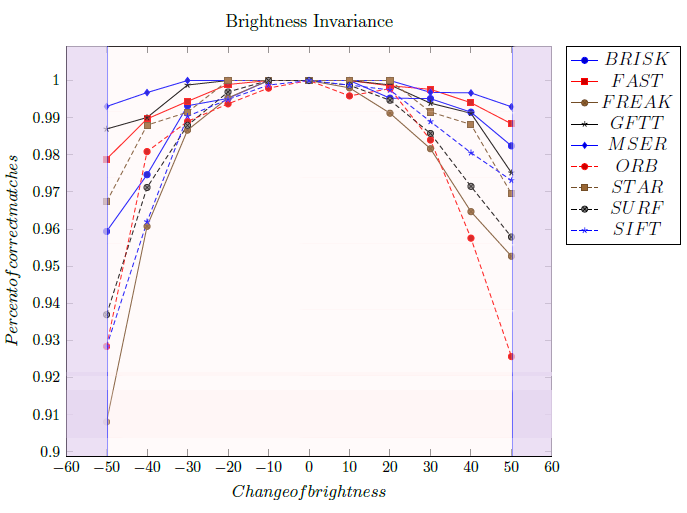
\includegraphics[scale=0.35]{images/bright-dummy}

\label{graph:brightresultpres}
\end{figure}

\end{frame}


\subsection{An�lise de Tempo}


\renewcommand{\gtype}{time}

\renewcommand{\maxy}{3000}
\renewcommand{\miny}{-155}



\renewcommand{\ylimit}{200}
\renewcommand{\ylabel}{Time(Ms)}


\begin{frame}
%scale
\begin{figure}[H]
\centering
\begin{tikzpicture}
	\pgfplotsset{small}
	%scale
\begin{axis}
	[
	   width=\graphwidth\textwidth,
      ylabel=$\ylabel$, % Set the labels
    xlabel=$Scale Factor$,
	legend entries={$BRISK$,$FAST$,$FREAK$,$GFTT$,$MSER$,$ORB$,$STAR$,$SURF$,$SIFT$},
	legend pos=outer north east,
	title= Robustness to scaling
    ]
	\addplot table [x=Argument, y=BRISK    , col sep=comma]	{graphs/scale-all-\gtype.csv}; 
	\addplot table [x=Argument, y=FAST     , col sep=comma]	{graphs/scale-all-\gtype.csv}; 
	\addplot table [x=Argument, y=FREAK    , col sep=comma]	{graphs/scale-all-\gtype.csv}; 
	\addplot table [x=Argument, y=GFTT     , col sep=comma]	{graphs/scale-all-\gtype.csv};
	 \addplot table [x=Argument, y=MSER     , col	sep=comma]	{graphs/scale-all-\gtype.csv};
	  \addplot table [x=Argument, y=ORB      , col sep=comma]	{graphs/scale-all-\gtype.csv}; 
	\addplot table [x=Argument, y=STAR     , col sep=comma]	{graphs/scale-all-\gtype.csv}; 
	\addplot table [x=Argument, y=SURF     , col sep=comma]	{graphs/scale-all-\gtype.csv}; 
	\addplot table [x=Argument, y=SIFT     , col sep=comma]	{graphs/scale-all-\gtype.csv}; 
	
	%eixo horizontal
	\addplot[red,sharp plot,update limits=false] coordinates{(\miny,\ylimit)
	(\maxx,\ylimit)}; 
	\fill [opacity=0.4,red!25] (axis cs:\miny,\ylimit) rectangle (axis
	cs:\maxx,\maxy);
	
	
	%eixo vertical
	\addplot[blue,sharp plot,update limits=false] coordinates {(\minscale,\miny)(\minscale,\maxy)} ;
		\fill [opacity=0.4,blue!25] (axis cs:\minx,\miny) rectangle (axis		cs:\minscale,\maxy);
	
	\addplot[blue,sharp plot,update limits=false] coordinates {(\maxscale,\miny)	(\maxscale,\maxy)} ;
	\fill [opacity=0.4,blue!25] (axis cs:\maxscale,\miny) rectangle (axis	cs:\maxx,\maxy);
	
\end{axis}
\end{tikzpicture}


\label{graph:scaleresulttime}

\end{figure}

\end{frame}

\begin{frame}
%rotation
\begin{figure}[H]
\centering
\begin{tikzpicture}
	\pgfplotsset{small}
\begin{axis}
	[
	   width=\graphwidth\textwidth,
      ylabel=$\ylabel$, % Set the labels
    xlabel=$Angle(Degree)$,
	legend entries={$BRISK$,$FAST$,$FREAK$,$GFTT$,$MSER$,$ORB$,$STAR$,$SURF$,$SIFT$},
	legend pos=outer north east,
	title= Rotation Invariance 
    ]
	\addplot table [x=Argument, y=BRISK    , col sep=comma]	{graphs/rot-all-\gtype.csv}; 
	\addplot table [x=Argument, y=FAST     , col sep=comma]	{graphs/rot-all-\gtype.csv}; 
	\addplot table [x=Argument, y=FREAK    , col sep=comma]	{graphs/rot-all-\gtype.csv}; 
	\addplot table [x=Argument, y=GFTT     , col sep=comma]	{graphs/rot-all-\gtype.csv};
\addplot table [x=Argument, y=MSER     , col	sep=comma]	{graphs/rot-all-\gtype.csv}; 
\addplot table [x=Argument, y=ORB      , col sep=comma]	{graphs/rot-all-\gtype.csv}; 
	\addplot table [x=Argument, y=STAR     , col sep=comma]	{graphs/rot-all-\gtype.csv}; 
	\addplot table [x=Argument, y=SURF     , col sep=comma]	{graphs/rot-all-\gtype.csv}; 
	\addplot table [x=Argument, y=SIFT     , col sep=comma]	{graphs/rot-all-\gtype.csv}; 

	
	%eixo horizontal
	\addplot[red,sharp plot,update limits=false] coordinates{(-100,\ylimit)
	(400,\ylimit)}; 
	\fill [opacity=0.4,red!25] (axis cs:-100,\ylimit) rectangle (axis
	cs:400,\maxy);
	
	
		%eixo vertical
	\addplot[blue,sharp plot,update limits=false] coordinates {(\minangle,-100)
	(\minangle,\maxy)} ;
		\fill [opacity=0.4,blue!25] (axis cs:-100,-100) rectangle (axis
		cs:\minangle,\maxy);
	
	\addplot[blue,sharp plot,update limits=false] coordinates {(\maxangle,-100)
	(\maxangle,\maxy)} ;
	\fill [opacity=0.4,blue!25] (axis cs:\maxangle,-100) rectangle (axis
	cs:400,\maxy);

	
\end{axis}
\end{tikzpicture}


\label{graph:rotresulttime}

\end{figure}

\end{frame}

\begin{frame}
%blur
\begin{figure}[H]
\centering
\begin{tikzpicture}
	\pgfplotsset{small}
\begin{axis}
	[
	   width=\graphwidth\textwidth,
      ylabel=$\ylabel$, % Set the labels
    xlabel=$Kernel size$,
	legend entries={$BRISK$,$FAST$,$FREAK$,$GFTT$,$MSER$,$ORB$,$STAR$,$SURF$,$SIFT$},
	legend pos=outer north east,
	title= Robustness to blur
    ]
	\addplot table [x=Argument, y=BRISK    , col sep=comma]	{graphs/blur-all-\gtype.csv}; 
	\addplot table [x=Argument, y=FAST     , col sep=comma]	{graphs/blur-all-\gtype.csv}; 
	\addplot table [x=Argument, y=FREAK    , col sep=comma]	{graphs/blur-all-\gtype.csv}; 
	\addplot table [x=Argument, y=GFTT     , col sep=comma]	{graphs/blur-all-\gtype.csv};
	 \addplot table [x=Argument, y=MSER     , col	sep=comma]	{graphs/blur-all-\gtype.csv}; 
	 \addplot table [x=Argument, y=ORB      , col sep=comma]	{graphs/blur-all-\gtype.csv}; 
	\addplot table [x=Argument, y=STAR     , col sep=comma]	{graphs/blur-all-\gtype.csv}; 
	\addplot table [x=Argument, y=SURF     , col sep=comma]	{graphs/blur-all-\gtype.csv}; 
	\addplot table [x=Argument, y=SIFT     , col sep=comma]	{graphs/blur-all-\gtype.csv}; 
	
	%eixo horizontal
	\addplot[red,sharp plot,update limits=false] coordinates{(\minx,\ylimit)
	(\maxx,\ylimit)}; 
	\fill [opacity=0.4,red!25] (axis cs:\minx,\ylimit) rectangle (axis
	cs:\maxx,\maxy);

				%eixo vertical
	\addplot[blue,sharp plot,update limits=false] coordinates
	{(\minblur,\miny)(\minblur,\maxy)} ; \fill [opacity=0.4,blue!25] (axis
	cs:\minx,\miny) rectangle (axis cs:\minblur,\maxx);
	
	\addplot[blue,sharp plot,update limits=false] coordinates
	{(\maxblur,\miny)(\maxblur,\maxy)} ; \fill [opacity=0.4,blue!25] (axis
	cs:\maxblur,\miny) rectangle (axis cs:\maxx,\maxy);


\end{axis}
\end{tikzpicture}


\label{graph:blurresulttime}

\end{figure}

\end{frame}


\begin{frame}
%bright
\begin{figure}[H]
\centering
\begin{tikzpicture}
	\pgfplotsset{small}
\begin{axis}
	[
	   width=\graphwidth\textwidth,
      ylabel=$\ylabel$, % Set the labels
    xlabel=$Change of brightness$,
	legend entries={$BRISK$,$FAST$,$FREAK$,$GFTT$,$MSER$,$ORB$,$STAR$,$SURF$,$SIFT$},
	legend pos=outer north east,
	title= Brightness Invariance 
    ]
	\addplot table [x=Argument, y=BRISK    , col sep=comma]	{graphs/bright-all-\gtype.csv}; 
	\addplot table [x=Argument, y=FAST     , col sep=comma]	{graphs/bright-all-\gtype.csv}; 
	\addplot table [x=Argument, y=FREAK    , col sep=comma]	{graphs/bright-all-\gtype.csv}; 
	\addplot table [x=Argument, y=GFTT     , col sep=comma]	{graphs/bright-all-\gtype.csv}; 
	\addplot table [x=Argument, y=MSER     , col sep=comma]	{graphs/bright-all-\gtype.csv}; 
	\addplot table [x=Argument, y=ORB      , col sep=comma]	{graphs/bright-all-\gtype.csv}; 
	\addplot table [x=Argument, y=STAR     , col sep=comma]	{graphs/bright-all-\gtype.csv}; 
	\addplot table [x=Argument, y=SURF     , col sep=comma]	{graphs/bright-all-\gtype.csv}; 
	\addplot table [x=Argument, y=SIFT     , col sep=comma]	{graphs/bright-all-\gtype.csv}; 
	
	%eixo horizontal
	\addplot[red,sharp plot,update limits=false] coordinates{(\minx,\ylimit)
	(\maxx,\ylimit)}; 
	\fill [opacity=0.4,red!25] (axis cs:\minx,\ylimit) rectangle (axis
	cs:\maxx,\maxy);
		
	
						%eixo vertical
	\addplot[blue,sharp plot,update limits=false] coordinates
	{(\minbright,\miny)(\minbright,\maxy)} ; \fill [opacity=0.4,blue!25] (axis
	cs:\minx,\miny) rectangle (axis cs:\minbright,\maxy);
	
	\addplot[blue,sharp plot,update limits=false] coordinates
	{(\maxbright,\miny)(\maxbright,\maxy)} ; \fill [opacity=0.4,blue!25] (axis
	cs:\maxbright,\miny) rectangle (axis cs:\maxx,\maxy);
		
	
\end{axis}
\end{tikzpicture}


\label{graph:brightresulttime}
\end{figure}

\end{frame}



\subsection{Sele��o da T�cnica}
\begin{frame}
\frametitle{Sele��o da T�cnica}

\definecolor{Gray}{gray}{0.85}
\newcolumntype{a}{>{\columncolor{Gray}}c}

 \begin{table}[H]
  \centering
  \caption{Decis�o de t�cnica a utilizar}
\label{table:techdecision}
  \resizebox{\textwidth}{!}{  
\begin{tabular}{ | l | l | l | l | a | l | a | l | l | l | }
\hline
	 & BRISK & FAST & FREAK & GFTT & MSER & ORB & STAR & SURF & SIFT \\ \hline
	Precis�o Escala &  &  & X & X &  & X &  &  &  \\ \hline
	Precis�o Rota��o & X & X & X & X & X & X & X & X & X \\ \hline
	Precis�o Blur &  & X & X & X & X & X & X & X & X \\ \hline
	Precis�o Ilumina��o & X & X & X & X & X & X & X & X & X \\ \hline
	Tempo Escala & X &  &  & X &  & X & X &  &  \\ \hline
	Tempo Rota��o & X &  &  & X &  & X & X &  &  \\ \hline
	Tempo Blur & X &  &  & X &  & X & X &  &  \\ \hline
	Tempo Ilumina��o & X &  &  & X &  & X & X &  &  \\ \hline
\end{tabular}
}

\end{table}

\end{frame}



